\section{Performance Degradtion Detection}

\begin{frame}
    \vfill
    \centering
    \begin{beamercolorbox}[sep=8pt,center,shadow=true,rounded=true]{title}
    \usebeamerfont{title}\insertsectionhead\par%
    \end{beamercolorbox}
    \vfill
\end{frame}

\begin{frame}
    \frametitle{Challenges}
    \begin{itemize}
        \item Imbalanced: For example, 83.5\% of the 16,868 HSPAP measurements for ISP Mobilis are from one user. If those measurements are excluded, the median RTT can decrease from 332ms to 219ms.
        \begin{itemize}
            \item normal association rules method bias to the performance of the dominating user.
        \end{itemize}
        \item Sparse: Although the total number of observations is huge, records for each combination of features can be very small.
        \begin{itemize}
            \item it's impossible to model the normal performance for all combinations of features separately.
        \end{itemize}
        \item Large: We need a scalable method to process the increasingly large data.
    \end{itemize}
\end{frame}

\begin{frame}
    \frametitle{Our Method\footnote{For more detailed description of our method we refer interested readers to attend IWQoS on 24-25 June 2019, Phoenix, AZ, USA or read the proceedings.}}
    \begin{enumerate}
        \item Based on the famous association rules mining method, the Apriori algorithm.
        \item We filter each candidate rule to ensure no more than half of the supporting records have the same feature.
        \item We identify performance degradtion events by comparing the meadian RTT of the supporting records for one candidate rule and a subset of it.
        \begin{itemize}
            \item For example, median RTT of LTE records is 73 in our data, while the RTT of the records that use LTE and linux kernel 3.10.49 has a median of 340.
        \end{itemize}
        \item Use Hypothesis test to verify that the supporting data cannot be split further.
    \end{enumerate}
\end{frame}

% \begin{frame}
%     \frametitle{Implementation Details}
%
% \end{frame}

\begin{frame}
    \frametitle{Evaluation}
    \begin{enumerate}
        \item Low false positive rate in random data
        \begin{itemize}
            \item We randomly shuffle the RTT of the records.
            \item We mathmatically proved that the probability of our methods thinking there is anomalies are very small in our configuration.
        \end{itemize}
    \end{enumerate}
\end{frame}

\begin{frame}
    \frametitle{Evaluation}
    \begin{enumerate}
        \item Low false positive rate in random data
        \item Real world case of Google Germany
    \end{enumerate}
    \vskip 1em
    \centering
    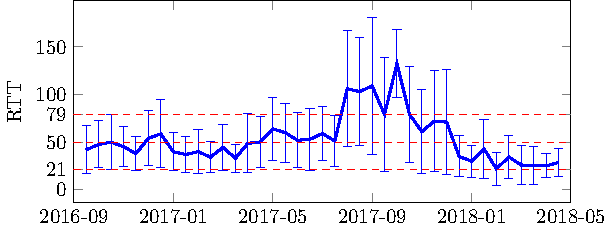
\includegraphics[width=.65\textwidth]{fig/case1.pdf}
\end{frame}

\begin{frame}
    \frametitle{Evaluation}
    \begin{enumerate}
        \item Low false positive rate in random data
        \item Real world case of Google Germany
        \item Real world case of Microsoft Office Mobile
    \end{enumerate}
    \vskip 1em
    \centering
    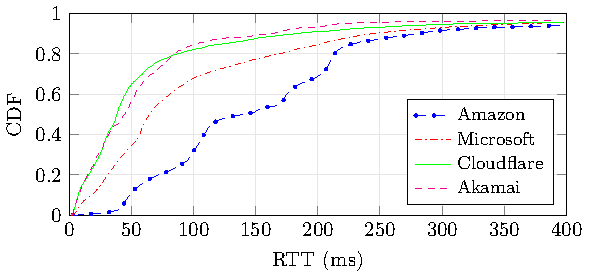
\includegraphics[width=.65\textwidth]{fig/case2.pdf}
\end{frame}
